\documentclass[man]{apa6}
\usepackage{lmodern}
\usepackage{amssymb,amsmath}
\usepackage{ifxetex,ifluatex}
\usepackage{fixltx2e} % provides \textsubscript
\ifnum 0\ifxetex 1\fi\ifluatex 1\fi=0 % if pdftex
  \usepackage[T1]{fontenc}
  \usepackage[utf8]{inputenc}
\else % if luatex or xelatex
  \ifxetex
    \usepackage{mathspec}
  \else
    \usepackage{fontspec}
  \fi
  \defaultfontfeatures{Ligatures=TeX,Scale=MatchLowercase}
\fi
% use upquote if available, for straight quotes in verbatim environments
\IfFileExists{upquote.sty}{\usepackage{upquote}}{}
% use microtype if available
\IfFileExists{microtype.sty}{%
\usepackage{microtype}
\UseMicrotypeSet[protrusion]{basicmath} % disable protrusion for tt fonts
}{}
\usepackage{hyperref}
\hypersetup{unicode=true,
            pdftitle={Introduction Draft},
            pdfauthor={Karen Santamaria, Yifan Ma, Caroline Li, \& Jane Bang},
            pdfborder={0 0 0},
            breaklinks=true}
\urlstyle{same}  % don't use monospace font for urls
\usepackage{graphicx,grffile}
\makeatletter
\def\maxwidth{\ifdim\Gin@nat@width>\linewidth\linewidth\else\Gin@nat@width\fi}
\def\maxheight{\ifdim\Gin@nat@height>\textheight\textheight\else\Gin@nat@height\fi}
\makeatother
% Scale images if necessary, so that they will not overflow the page
% margins by default, and it is still possible to overwrite the defaults
% using explicit options in \includegraphics[width, height, ...]{}
\setkeys{Gin}{width=\maxwidth,height=\maxheight,keepaspectratio}
\IfFileExists{parskip.sty}{%
\usepackage{parskip}
}{% else
\setlength{\parindent}{0pt}
\setlength{\parskip}{6pt plus 2pt minus 1pt}
}
\setlength{\emergencystretch}{3em}  % prevent overfull lines
\providecommand{\tightlist}{%
  \setlength{\itemsep}{0pt}\setlength{\parskip}{0pt}}
\setcounter{secnumdepth}{0}
% Redefines (sub)paragraphs to behave more like sections
\ifx\paragraph\undefined\else
\let\oldparagraph\paragraph
\renewcommand{\paragraph}[1]{\oldparagraph{#1}\mbox{}}
\fi
\ifx\subparagraph\undefined\else
\let\oldsubparagraph\subparagraph
\renewcommand{\subparagraph}[1]{\oldsubparagraph{#1}\mbox{}}
\fi

%%% Use protect on footnotes to avoid problems with footnotes in titles
\let\rmarkdownfootnote\footnote%
\def\footnote{\protect\rmarkdownfootnote}


  \title{Introduction Draft}
    \author{Karen Santamaria\textsuperscript{1}, Yifan Ma\textsuperscript{1}, Caroline Li\textsuperscript{1}, \& Jane Bang\textsuperscript{1}}
    \date{}
  
\shorttitle{SDS/PSY 365}
\affiliation{
\vspace{0.5cm}
\textsuperscript{1} Smith College}
\usepackage{csquotes}
\usepackage{upgreek}
\captionsetup{font=singlespacing,justification=justified}

\usepackage{longtable}
\usepackage{lscape}
\usepackage{multirow}
\usepackage{tabularx}
\usepackage[flushleft]{threeparttable}
\usepackage{threeparttablex}

\newenvironment{lltable}{\begin{landscape}\begin{center}\begin{ThreePartTable}}{\end{ThreePartTable}\end{center}\end{landscape}}

\makeatletter
\newcommand\LastLTentrywidth{1em}
\newlength\longtablewidth
\setlength{\longtablewidth}{1in}
\newcommand{\getlongtablewidth}{\begingroup \ifcsname LT@\roman{LT@tables}\endcsname \global\longtablewidth=0pt \renewcommand{\LT@entry}[2]{\global\advance\longtablewidth by ##2\relax\gdef\LastLTentrywidth{##2}}\@nameuse{LT@\roman{LT@tables}} \fi \endgroup}


\DeclareDelayedFloatFlavor{ThreePartTable}{table}
\DeclareDelayedFloatFlavor{lltable}{table}
\DeclareDelayedFloatFlavor*{longtable}{table}
\makeatletter
\renewcommand{\efloat@iwrite}[1]{\immediate\expandafter\protected@write\csname efloat@post#1\endcsname{}}
\makeatother

\authornote{

Correspondence concerning this article should be addressed to Karen Santamaria, 1 Chapin Way, Unit 7766, Northampton, MA 01063. E-mail: \href{mailto:sanmakaren@gmail.com}{\nolinkurl{sanmakaren@gmail.com}}}



\begin{document}
\maketitle

\begin{figure}

{\centering 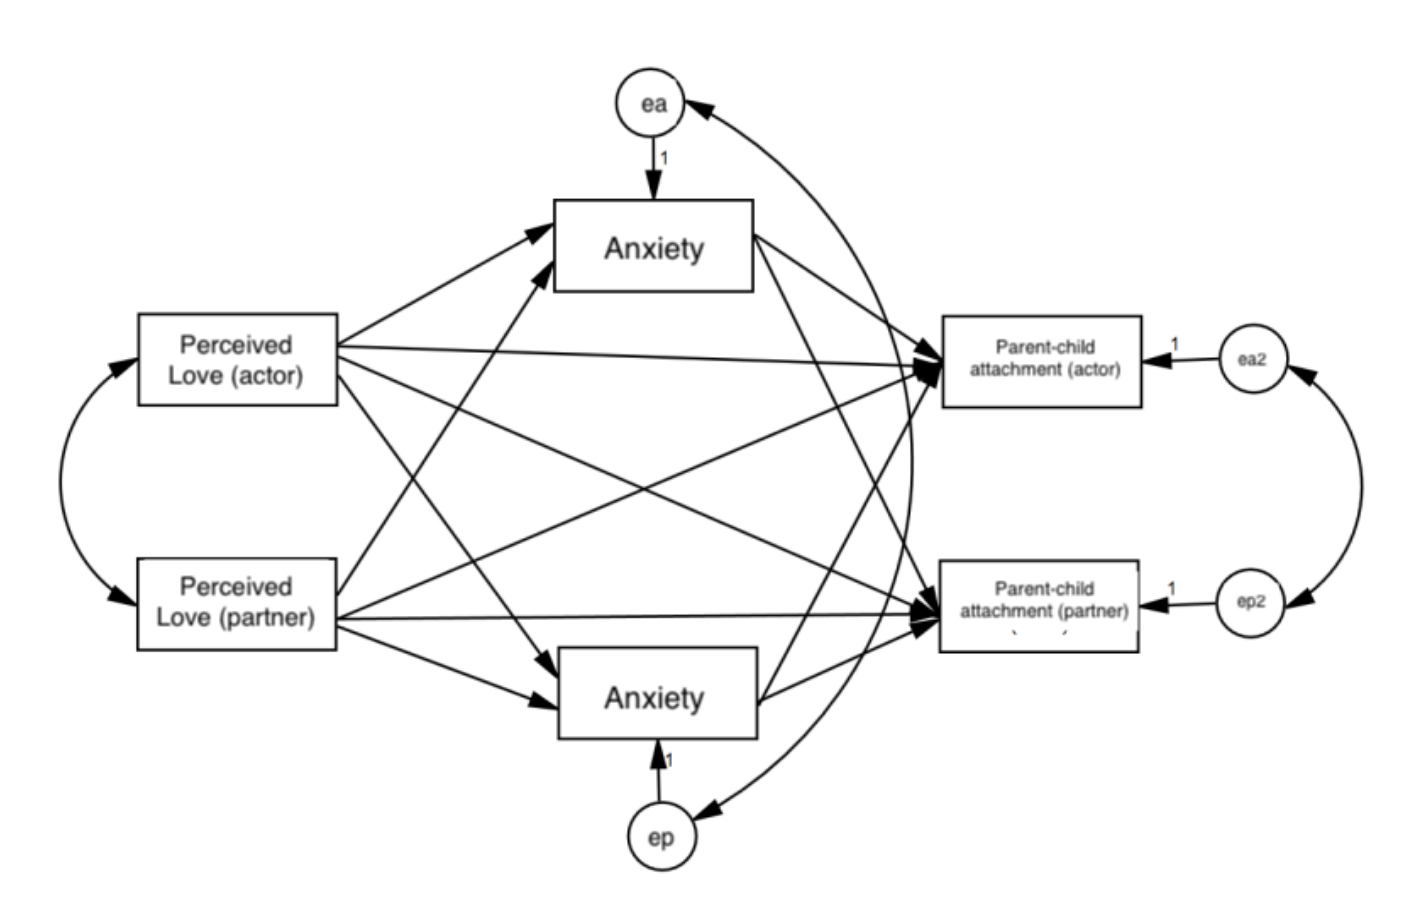
\includegraphics[width=500px]{figure1} 

}

\caption{caption}\label{fig:unnamed-chunk-1}
\end{figure}

\begin{figure}

{\centering 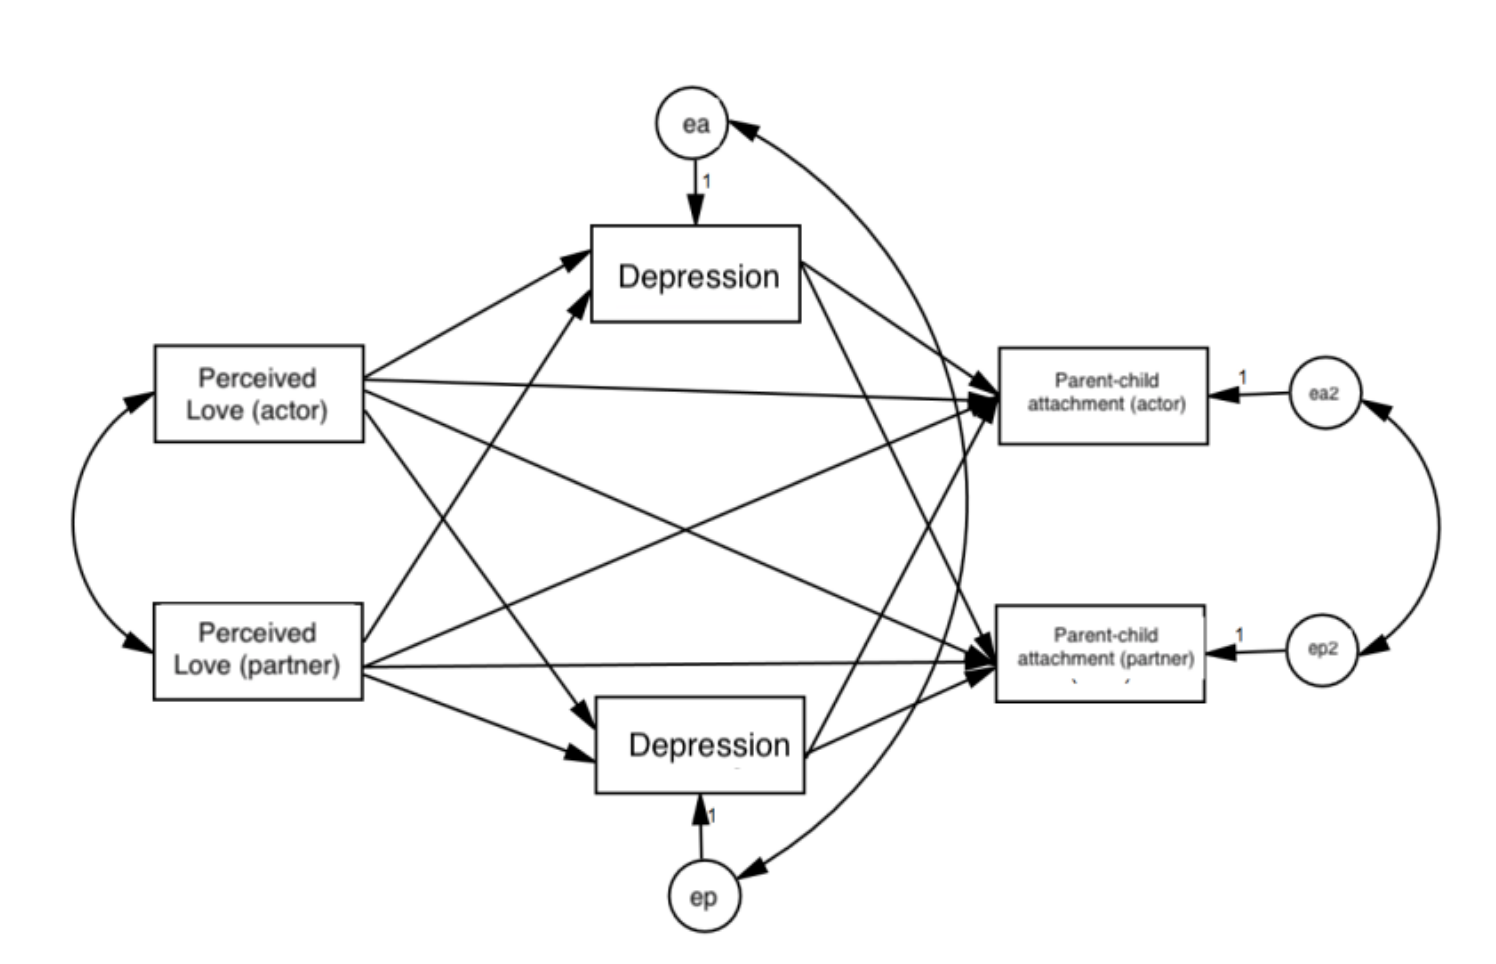
\includegraphics[width=500px]{figure2} 

}

\caption{caption}\label{fig:unnamed-chunk-2}
\end{figure}

\hypertarget{results}{%
\section{Results}\label{results}}

\hypertarget{analysis-strategy}{%
\subsection{Analysis Strategy}\label{analysis-strategy}}

We hypothesized that the individuals' perception of love and their partner's perception of love in their relationship would affect the parent-child relationship positively and associations would become stronger over time (hypothesis 1). We also hypothesized that the correlation between love and parent-child attachment would be different across family types (hypothesis 2). Furthermore, we hypothesized that depressive and anxiety symptoms play mediating roles in the association between love and attachment (hypotheses 3 and 4). We used multilevel modeling and the Actor-Partner Interdependence Model (APIM; Kenny, Kashy, \& Cook, 2006) to test these hypotheses. The APIM (see Figure 1\&2) does THIS, and THIS. Most importantly, it does THIS and THIS. \textless{}- something about the correlated errors to account for the non-independence.

We first used the following explanatory variables: 1) actor's perception of love in the relationship, 2) partner's perception of love in the relationship, 4) time. The response variable was actor's attachment. To test if anxiety (of the actor) mediates love we used the Monte Carlo method (Tofighi \& MacKinnon, 2011) for assessing mediation which created confidence intervals for indirect effects.

\hypertarget{main-results}{%
\subsection{Main Results}\label{main-results}}

\hypertarget{hyp1}{%
\subsubsection{Hyp1:}\label{hyp1}}

In our first model, there was a statistically significant effect of the individuals' perception of love on the perceived parent-child attachment for that individual, such that the higher the perception of love the more the person perceived that they were attached to their children , b = 0.11, SE = 0.019 , p = 0.000. Nevertheless, a person's partner's perception of love in their relationship did not show statistical significant on neither themselves's nor their partner's perceived parent-child attachment. We also found that time was not a statistically significant moderator for the correlation between love and attachment, such as the correlation between love and attachment for a person at time point one does not predict the correlation between love and attachment for a person at the following time point.

\hypertarget{hyp2}{%
\subsubsection{Hyp2:}\label{hyp2}}

We did not find the interaction of different family types on the correlation between love and parent-child attachment with respect to time point statistically significant.

\hypertarget{hyp3}{%
\subsubsection{Hyp3:}\label{hyp3}}

In our third model, there was a statistically significant actor effect of anxiety on attachment, such that the higher the person's anxiety the less the person perceived that they are attached to their children , b = -0.31, SE = 0.041, p = 0.000.
We also found that the relationship between love and attachment is (positively/negatively) mediated by anxiety. b = 0.27, SE = 0.045, p = .002.

\newpage

\hypertarget{references}{%
\section{References}\label{references}}

\begingroup
\setlength{\parindent}{-0.5in}
\setlength{\leftskip}{0.5in}

\hypertarget{refs}{}
\leavevmode\hypertarget{ref-monte}{}%
Tofighi, D., \& MacKinnon, D. P. (2011). RMediation: An r package for mediation analysis confidence intervals. \emph{Behavior Research Methods}, \emph{43}(3), 692--700.

\endgroup


\end{document}
